\chapter[Fundamentação Teórica]{Fundamentação Teórica}

Neste capítulo serão apresentados os componentes utilizados durante o desenvolvimento do trabalho, assim como suas 
principais características e motivos de cada escolha. Componentes relacionados diretamente a montagem física do sistema
serão abordados de forma sucinta, pois o escopo do trabalho se dispões a apresentar um \textit{Framework} de desenvolvimento
que não se limita aos circuitos e componentes utilizados, por outro lado é importante pontuar alguns detalhes quanto a 
parte de implementação dos códigos que serão vitais para o entendimento da abrangência do modelo utilizado.

\section{Circuitos Eletrohidráulicos e Eletropneumáticos}

\begin{figure}[htb]
    \begin{center}
	    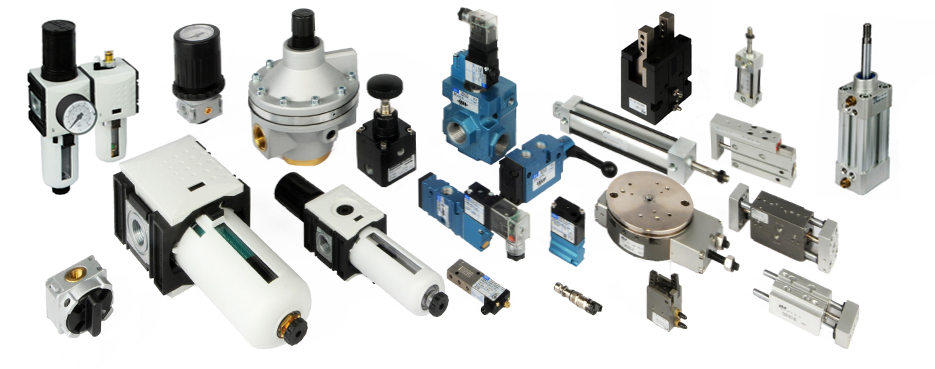
\includegraphics[scale=0.5]{figs/set-pneumatica.jpg}
	\end{center}
	\caption{Exemplo de componentes pneumáticos.} 
\end{figure}

No contexto da Engenharia Mecatrônica e da automação no geral, uma das principais tecnologias utilizadas na solução de
problemas de diferentes áreas são os circuitos de comando hidráulicos e pneumáticos, seu amplo uso já de longo período e
sua capacidade de ser implementada em diferentes campos fazem com que esta ferramenta possua ampla documentação e suporte
de uma estabelecida cadeia de suprimentos, com os mais diversos tipos de componentes. Este consolidado status garante 
que estes circuitos sejam um tópico amplamente abordado durante a formação do engenheiro, e como em qualquer outra 
ferramenta neste contexto são desenvolvidos diversos modelos e métodos que auxiliam em sua implementação. 

\subsection{Métodos de Representação e Simulação}

Uma das ferramentas mais importantes que garantem a circuitos hidráulicos e pneumáticos a posição mencionada acima é a 
existência de uma simbologia bastante sólida para os cada vez mais complexos sistemas utilizados na industria. Esta simbologia,
instituida primeiramente pela ISO 1219:1997 \cite{ISO1219:1997}, mas substituída algumas vezes logo depois até atingir a
estrutura atual, na qual seu escopo foi dividido em três partes:

\begin{figure}[htb]
    \begin{center}
	    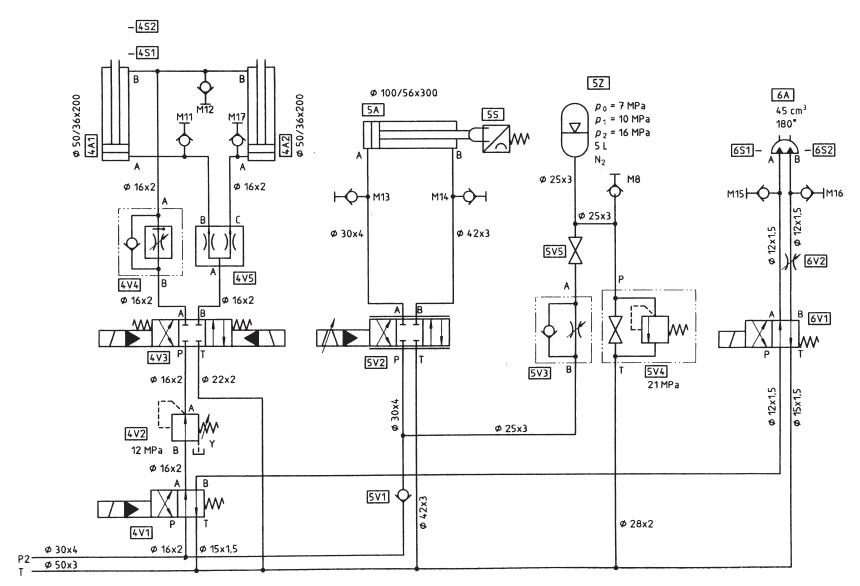
\includegraphics[scale=0.5]{figs/std-example.png}
	\end{center}
	\caption{Exemplo de diagrama proposto na norma.} 
\end{figure}

\begin{itemize}

    \item ISO 1219-1:20012 \cite{ISO1219-1:2012}: que versa diretamente sobre os símbolos utilizados nos diagramas de 
    forma isolada (esta parte recebeu em 2016 a inclusão da emenda AMD 1:2016 \cite{ISO1219-1:2012/AMD-1:2016}) 
    \item ISO 1219-2:20012 \cite{ISO1219-2:2012}: que, por sua vez, versa sobre as características construtivas de 
    circuitos conexões, agrupamento e entre outros. 
    \item ISO 1219-3:20016 \cite{ISO1219-3:2016}: que versa sobre a utilização de módulos, isto é, modelos de representação
    de pequenos agrupamentos utilizados repetitivamente em circuitos muito grandes.

\end{itemize}

A partir desta simbologia podemos criar uma série de \textit{softwares} de simulação capazes de auxiliar-nos na 
implementação dos mais diversos sistemas, como o FluidSIM\textregistered~ e o Automation Studio, onde podemos executar
versões virtuais dos ambientes reais, e observar os resultados. 

\subsection{Ladder}

Apesar do ambiente altamente robusto descrito acima, o crescimento da complexidade dos problemas abordados no meio da 
automação industrial ainda tem se mostrado como um grande desafio. Neste contexto um segundo tópico que também tem função 
importante é o desenvolvimento de métodos que pudessem auxiliar no desenvolvimento dá lógica, sendo em um primeiro momento
a inclusão dos diagramas de relés, de forma a ficarem estes componentes os principais responsáveis pelo comando; 
mas depois sendo substituído por \ac{CLP} um componente capaz de implementar via código as complicadas sequências de acionamento.
Os primeiros esforços no sentido de garantir um modelo padronizado neste sentido vieram da norma IEC 61131 que se dispunha
a trazer uma série de conceitos relacionados aos \ac{CLP}s em geral como apresentado logo no início do documento.

\begin{citacao}
    This Part of IEC 61131 applies to programmable controllers (PLC) and their associated 
    peripherals such as programming and debugging tools (PADTs), human-machine interfaces
    (HMIs), etc., which have as their intended use the control and command of machines and
    industrial processes.\cite{IEC-61131-1:2003}
\end{citacao}    

Entre todo o material apresentado na norma, a parte que mais interessa a este trabalho é a descrita na IEC 61131-3:2013 
em que são propostas quatro linguagens de programação: \ac{IL}, \ac{ST}, \ac{LD} e \ac{FBD} \cite{IEC-61131-3:2013} 
que tornavam simples a implementação de código nos \ac{CLP}s e, falando especificadamente dos códigos em \ac{LD} a 
linguagem foi construída de forma que estes códigos pudessem ser facilmente interpretados como um diagrama de relés.

\begin{citacao}
    A LD program enables the programmable controller to test and modify data by means of standardized
    graphic symbols. These symbols are laid out in networks in a manner similar to a “rung” of a relay
    ladder logic diagram. LD networks are bounded on the left and right by power rails.\cite{IEC-61131-3:2013}
\end{citacao}    

\begin{figure}[htb]
    \begin{center}
	    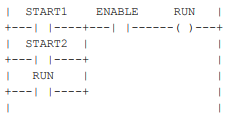
\includegraphics{figs/ladder-diag.png}
	\end{center}
	\caption{Exemplo de código Ladder proposto na norma.} 
\end{figure}

\subsection{GRAFCET}

Por fim, como último método de grande importância no desenvolvimento de circuitos hidráulicos e pneumáticos em geral, 
podemos mencionar o \ac{GRAFCET} já que este é um tipo de modelagem onde conseguimos representar de uma forma sequancial
modelos altamente complexos. Por ser baseado nas Redes de Petri o \ac{GRAFCET} é visto como um modelo com forte base
matemática comprovado pela teoria de grafos.

Apesar de ser um método para modelagem e dimensionamento de processos, alguns \ac{CLP}s aceitam o \ac{GRAFCET} como uma
linguagem de programação diretamente assim como previsto na norma IEC 60848:2013 \cite{IEC-60848:2013}, o que traz uma 
grande praticidade na implementação de processos longos, além de garantir uma maneira mais simples para entendimento dos 
processos permitindo que grandes times possam trabalhar no seu desenvolvimento.

\begin{figure}[htb]
    \begin{center}
	    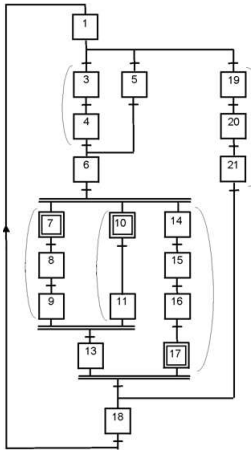
\includegraphics[scale=0.5]{figs/grafcet-diag.png}
	\end{center}
	\caption{Exemplo de código GRAFCET proposto na norma.} 
\end{figure}

\section{Computação em Nuvem}

Visto como uma das maiores \textit{buzzword}\footnote{Segundo o dicionário Cambridge: \textit{Buzzword} é uma palavra ou expressão de uma 
área de assunto particular que se tornou moda, porque tem sido muito usado \cite{buzzword-cam}} da atualidade e com uso 
ainda crescente. Porém, a definição de computação em nuvem é bastante vaga \cite{artigo-nuvem} em alguns casos sendo 
associada a virtualização de servidores, em outros casos a disponibilização de Infraestrutura como serviço (\ac{IaaS}) ou 
alguma das variações do "\textit{as a service}"; ou até em alguns casos uma referência a localização material dos grandes
\textit{Data Centers} sua disposição territorial e etc. Fato é que nem entre os próprios provedores destes serviços 
existe uma padronização, de como eles são disponibilizados; observando os três principais hoje vemos que a AWS\textregistered~
utiliza um modelo de \textit{server virtualization}, enquanto a Azure\textregistered~ se baseia no \ac{WAH} e o Google\textregistered~, por sua vez, segue o 
conceito de \textit{technique-specific sandbox} \cite{artigo-nuvem}.

No contexto deste trabalho considerar-se-á nuvem como um modelo de virtualização, no qual se delega toda a parte de 
infraestrutura computacional e podemos acessar os recursos desejados a partir de uma representação abstrata na maioria 
das vezes disponibilizadas a partir de uma interface via Internet. Conceito que apesar de gerar um grande barulho atualmente
não tem nada de novo, ao contrário, era uma dos conceitos já discutidos desde a concepção do \textit{Multics}, sistema 
operacional precursor do Unix e, portanto, do modelo seguido no GNU atual, como pode ser visto no paper de apresentação 
do projeto.

\begin{citacao}
It is important to recognize that the average user of the system will see no part of the segmentation and paging 
complexity described in the paper by Glaser et al. Instead he will see a virtual machine with many system characteristics 
which are convenient to him for writing either single programs or whole subsystems. \cite{multics-paper}
\end{citacao}

\section{O Protocolo MQTT}

Apresentado pela própria OASIS\textregistered~ como o protocolo padrão para a troca de mensagens \ac{IOT} o protocolo \ac{MQTT}
tem ganhado espaço em diversas aplicações por se mostrar como um modelo em que cada componente é capaz de controlar qual
tipo de informação ele pode transmitir e receber, o que é visto como um grande ganho do ponto de vista do \ac{IOT}; além 
disso, em uma rede \ac{MQTT} a entrada e saída de novos componentes em rede acontece de forma bastante simples, sem 
necessitar que o responsável pela rede refaça toda sua configuração.

Para implementar estes conceitos o protocolo utiliza a arquitetura \textit{publisher/subscriber} em que são definidos
uma série de tópicos e cada componente pode se cadastrar como publicador de um grupo de tópicos e subscritor de outro 
grupo de tópicos\footnote{Estes grupos não são exclusivos}. Assim, os servidores desta rede (ou \textit{Brokers} seguindo a terminologia
descrita no OASIS MQTTv5 Standard \cite{mqtt-std}) podem deixar a função de orquestradores da rede e se tornarem responsáveis
por rotear as mensagens transmitidas por cada tópico. Com o uso do \ac{MQTT}, temos um grande avanço no sentido de objetos
em rede autogerenciáveis, mais informações sobre o uso desta ferramenta em especifíco neste trabalho serão apresentadas 
mais a frente.

\begin{figure}[htb]
    \begin{center}
	    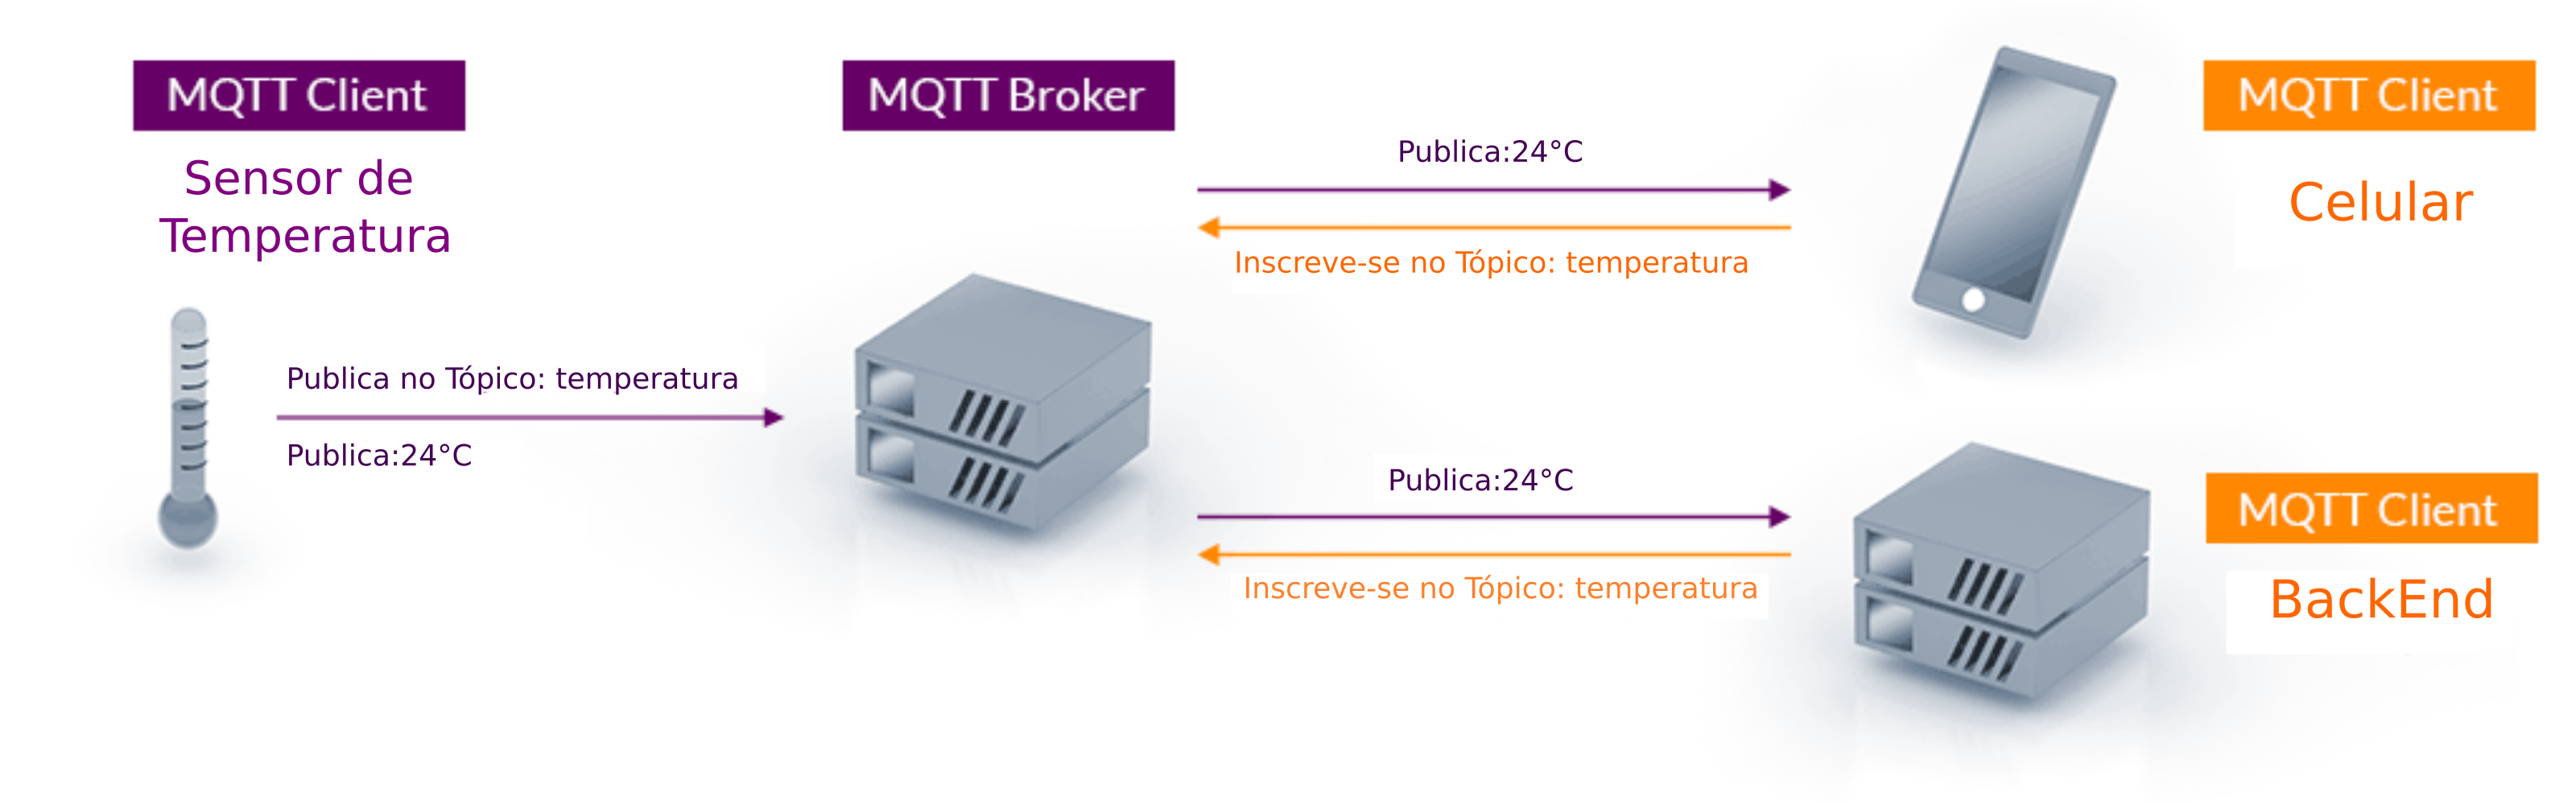
\includegraphics[scale=0.3]{figs/mqtt-publish-subscribe.png}
	\end{center}
	\caption{Diagrama representativo da arquitetura \ac{MQTT}.} 
\end{figure}

\section{Microcontroladores ESP32}

Tido como um dos principais microcontroladores para desenvolvimento \ac{IOT} os ESP tem uma grande vantagem em relação 
a uma gama de outros microcontroladores pois possuem módulos para comunicação \textit{wireless} embutidos no próprio
\textit{chip}, neste meio a família ESP32 apresenta-se, entre as linhas de produto ainda em desenvolvimento pela 
Expressif\textregistered~, como uma das mais completas apresentando como principais características:

\begin{itemize}
\item 2.4 GHz Wi­Fi + Bluetooth® + Bluetooth LE module
\item microprocessador Xtensa® dual­core 32­bit LX6
\item opções de: 4/8/16 MB memória flash
\item 26 GPIOs, com grande gama de periféricos disponíveis
\item Antena PCB na placa ou conector para antena externa
\end{itemize}

\subsection{Características do Componente}

Apesar de muitas pessoas entenderem os ESPs diretamente como uma placa de desenvolvimento, às vezes até como uma 
alternativa semelhante ao arduino, é importante fazer a distinção clara entre os dois componentes. Diferente 
do Arduino onde temos vários \ac{CI} com diferentes funções, no caso do ESP32 estamos falando de um \ac{SoC} responsável
por todas estas capacidades acima. Por outro lado, o fabricante disponibiliza em seu catálogo três modelos de encapsulamento
para o mesmo \textit{chip}, sendo eles: 

\begin{itemize}
    \item \textbf{ESP32 DOWD v3}, o próprio \ac{SoC}, sendo este o modelo mais simples e econômico para inclusão em produtos já de longo ciclo no 
    mercado, porém utilizar este componente diretamente no circuito exige um maior tempo dedicado ao \textit{design} da interface, uma 
    vez que ele traz consigo uma série de \textit{guidelines} a serem seguidos para sua instalação. \cite{datasheet-soc}
    \item \textbf{ESP32-WROOM-32E}, o módulo, sendo este o grande foco deste trabalho, é um módulo de fácil inclusão no \textit{design} de outras PCBs   
    possui já possui proteção térmica e de ruído, circuito para filtro da fonte de tensão, gerador de \textit{clock} e antena PCB inclusos. \cite{datasheet-modulo}
    \item \textbf{ESP32-DevKitC}, a placa de prototipagem, neste componente temos uma pinagem de simples acesso para as saídas do módulo de forma 
    que o uso de \textit{jumpers} fica simples, e também temos incluído botões para mudar o \textit{chip} para o modo de gravação, uma porta USB, e
    Leds indicadores de funcionamento.
\end{itemize}

\begin{figure}[htb]
    \begin{center}
	    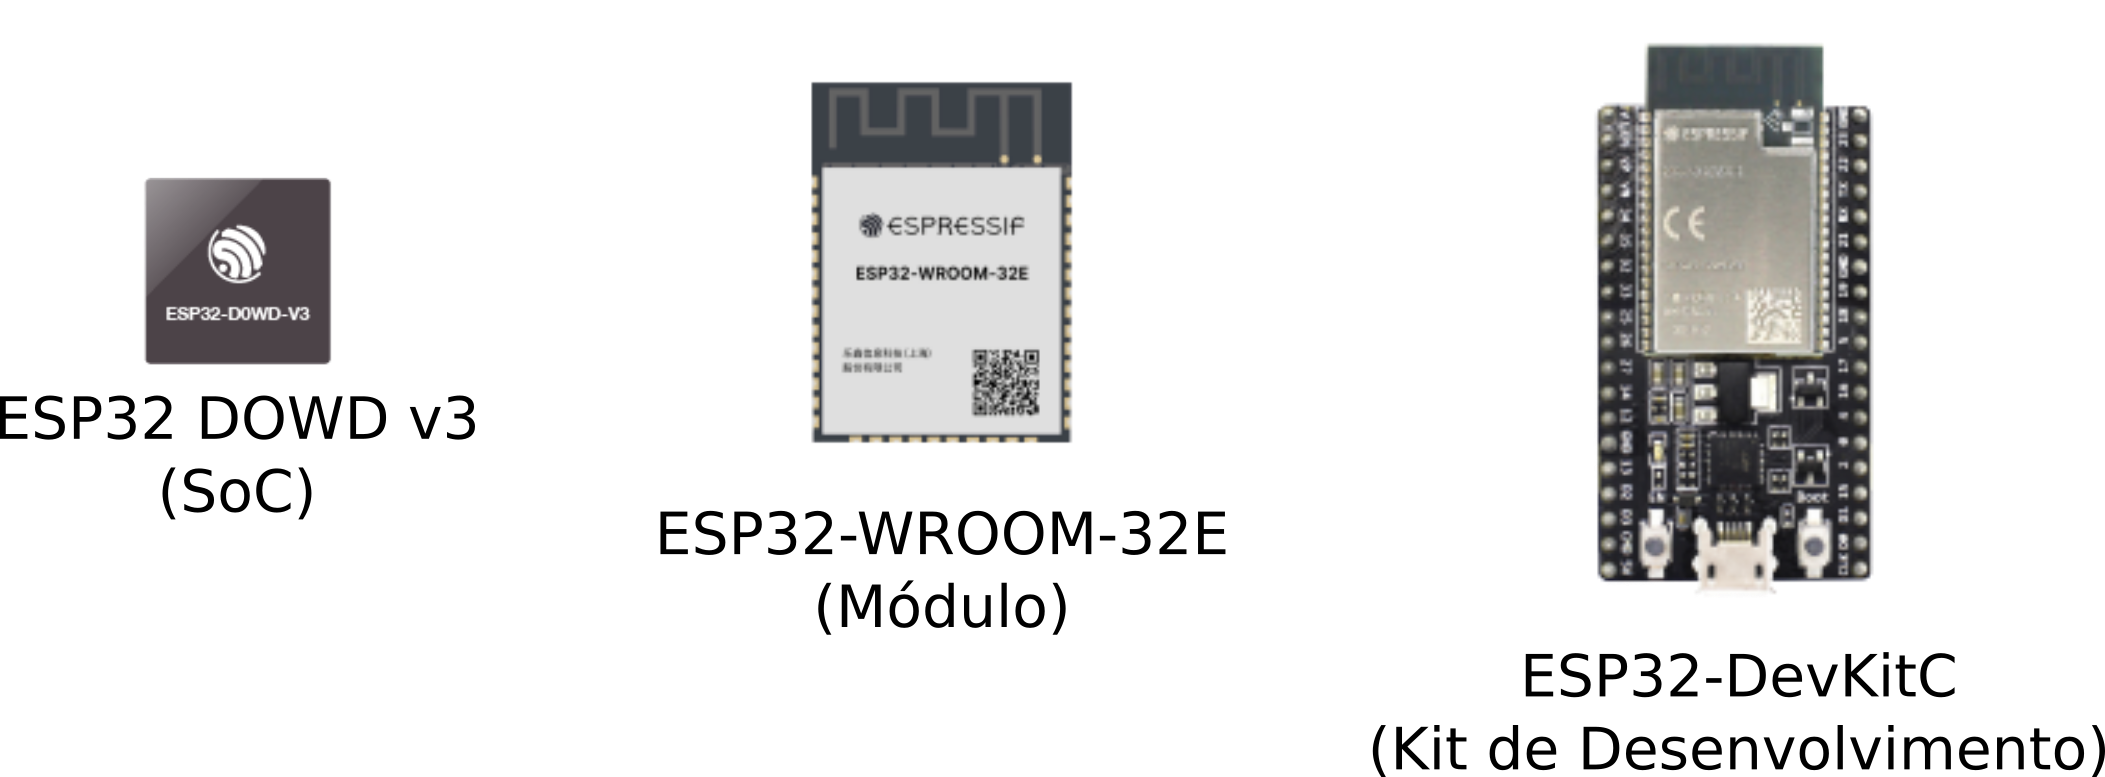
\includegraphics[scale=0.5]{figs/esp32-familia.png}
	\end{center}
	\caption{\label{fig:esp-fam} Distinção entre os componentes baseados no ESP32.} 
\end{figure}

Embora os experimentos deste trabalho tenham sido realizados com o ESP32-DevKitC, não existem restrições quanto ao seu uso também no módulo
ESP32-WROOM-32E, as representações esquemáticas destes componentes estão disponíveis respectivamente no Anexo \ref{ane:kit} e no Anexo \ref{ane:mod}.

\subsection{Ambiente de Desenvolvimento}

Outra característica importante dos ESP32 é que eles utilizam o \ac{ESP-IDF} o ambiente de desenvolvimento oficial 
disponibilizado pelo fabricante baseado \textit{FREERTOS}®. Um ambiente amplamente documentado com \textit{scripts} 
Python e Cmake que facilitam o processo de compilação e \textit{link} do \textit{firmware}, além disso do ponto de 
vista da compilação o \ac{ESP-IDF} utiliza versões oficiais do GCC com \textit{backend} específico para a a família de 
processadores Xtensa® LX6\footnote{Essa informação não abrange os ESP32-S2 ou ESP32-C3, estas séries de processadores
possuem versões diferentes do GCC (backend LX7, RISCV e etc.) assim como descrito no Github do \ac{MAPL}\cite{mapl-repo}};
e são, portanto, compatíveis com todas as linguagens suportadas no \textit{frontend} do GCC utilizado (C, C++, Objective-C,
FORTRAN, Go e etc).

\begin{figure}[htb]
    \begin{center}
	    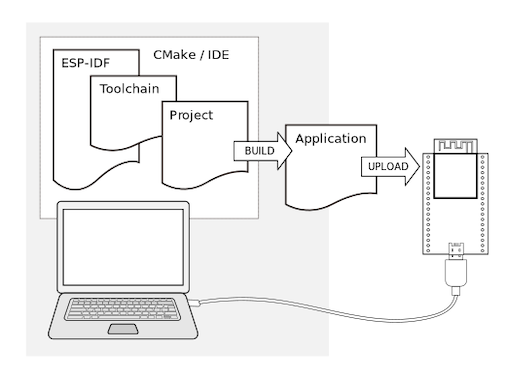
\includegraphics[scale=0.5]{figs/comp-flow.png}
	\end{center}
	\caption{Modelo \ac{ESP-IDF}.} 
\end{figure}

No momento da construção deste trabalho, a versão de suporte padrão para o \textit{framework} utilizava o GCC 5.3  com 
suporte máximo para o Std17\cite{suported-c}, assim como esperado de acordo com as informações de \textit{release} do GCC
5 \cite{gcc-5}. 

Optou-se, portanto, pela utilização em todos os códigos deste trabalho do C++17. O uso do C++ se justifica
porque o grande objetivo do trabalho é produzir uma plataforma de fácil entendimento. Por outro lado, o uso do padrão 17
se dá com o objetivo de seguir as recomendações do próprio \textit{release} disponível no site da GNU designando ente como
novo padrão para o compilador \cite{gcc-5}.


\section{A plataforma Raspberry PI\textregistered}

Uma plataforma que tem ganhado bastante notoriedade tanto nos assuntos que envolvem engenharia quanto na area da computação
são os Raspberry PI, um pouco diferente do que costuma-se ver em \textit{chips all-in-one} os Raspbery-PI se dispõe a 
ser um \textit{Desktop} completo com entradas para teclado, mouse, saídas de audio e video, se mostrando até como uma 
opção para uso pessoal. Estes componentes impressionam bastante por suas capacidades em um primeiro contato. Apesar 
de aparecerem associados a projetos \textit{open source} de várias formas, eles não o são; muito embora seja possível
encontrar muito sobre seu funcionamento, inclusive os desenhos esquemáticos, na própria documentação do fabricante. \cite{raspberry-pi}

\begin{figure}[htb]
    \begin{center}
	    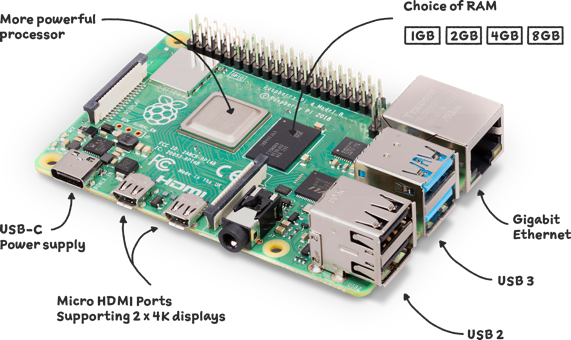
\includegraphics[scale=0.5]{figs/raspberry-pi-4.png}
	\end{center}
	\caption{Raspberry PI 4.} 
\end{figure}

Do ponto de vista de \textit{software}, os Raspberry PI possuem compatibilidade com uma série de \ac{SO} Linux o que 
faz destes componentes também uma opção interessante para a prototipagem de programas mais completos e que vão rodar 
sobre o ambiente de um \ac{SO}.

Apesar da Raspbery disponibilizar em seu site um \ac{SO} específico para uso nesta placa, capaz de extrair melhor 
desenpenho da mesma; no contexto do corrente trabalho o \ac{SO} utilizado foi a atual versão \ac{LTS} do Ubunto Server (22.04),
que por ser uma das versões mais utilizadas mundialmente em servidores garante que todos os códigos utilizados aqui podem 
ser portabilizados para servidores padrão, estejam eles em nuvem ou não. O passo a passo desta instalação pode ser 
encontrado em na página do fabricante. \cite{ubunto-inst}

\section{Mosquitto\textregistered~ Broker}

Desenvolvido pela Eclipse Foudation\textregistered~ o \textit{Broker} Eclipse Mosquitto, ou somente Mosquitto, é uma 
implementação de um \textit{Broker} \ac{MQTT} com interface de simples aprendimento, tanto para instalações locais,
quanto para aquelas feitas de forma remota. Além disso, o Mosquitto é conhecido por ser um programa que requer para 
seu funcionamento poucos recursos seja no âmbito do processamento ou no âmbito do espaço em memória.

Embora muito simples, o \textit{Broker} Mosquitto possui uma série de funções importantes que vão desde segurança via 
certificados x509 até a implementação do modo Bridge: Um modo de funcionamento onde as mensagens publicadas em um 
\textit{Broker} são repetidas em um ou mais espelhos, sendo o contrário também possível todas estas possíveis configurações
podem ser consultadas na documentação dos arquivos ".conf". \cite{mosq-doc}
 
